\documentclass[14pt, a4paper]{report}
\usepackage{mathtext}
\usepackage[T2A]{fontenc}
\usepackage[utf8]{inputenc}
\usepackage[russian]{babel}
\usepackage{multirow}
\usepackage{slashbox}
\usepackage{makecell}
\usepackage{graphicx}
\usepackage{physics}
\usepackage{amstext}
\usepackage{caption}
\usepackage{subcaption}
\usepackage{cmap}
\usepackage{float}
\usepackage{indentfirst}
\usepackage{romannum}
\usepackage{siunitx}

\usepackage[a4paper,
            		left=1in,
            		right=1in,
           		 top=1in,
            		bottom=1in,
            		footskip=.25in]{geometry}

\renewcommand{\thesection}{\arabic{section}.}
\renewcommand{\thesubsection}{\arabic{section}.\arabic{subsection}.}

\title{\textbf{Отчет о выполнении лабораторной работы 1.3 "Эффект Рамзауэра"}}
\author{Калашников Михаил, Б03-202}
\date{}

\begin{document}
\pagenumbering{arabic}
\maketitle

\textbf{Цель работы:}
Исследование энергетической зависимости вероятности рассеяния электронов атомами ксенона, определение энергии электронов, при которых наблюдается "просветление" ксенона, и оценивание размера его внешней электронной оболочки.
\newline

\section{Теоретические сведения}

Эффективным сечением реакции называется величина, характеризующая вероятность перехода системы двух сталкивающихся частиц в результате их рассеяния в определенное конечное состояние. Сечение $\sigma$ равно отношению числа $N$ таких переходов в единицу времени к плотности $nv$ потока рассеиваемых частиц.

\[\sigma=\frac{N}{nv}\]

\begin{figure}[H]
\centering
\begin{minipage}{.5\textwidth}
  \centering
  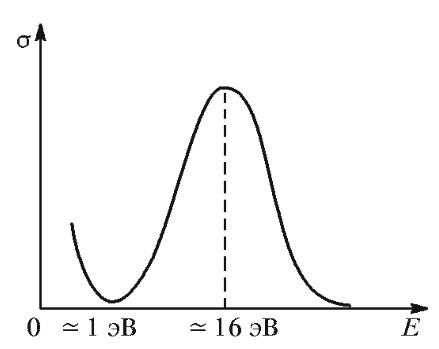
\includegraphics[width=.8\linewidth]{../images/513-1}
  \caption{Качественная картина результатов измерения упругого рассеяния электронов в аргоне}
\end{minipage}%
\begin{minipage}{.5\textwidth}
  \centering
  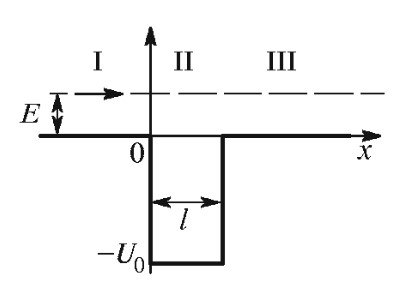
\includegraphics[width=.8\linewidth]{../images/513-2}
  \caption{Схематическое изображение прямоугольной потенциальной ямы, над которой пролетаем частица с энергией E}
\end{minipage}
\end{figure}

Объяснение эффекта, приведенного на рисунке выше, требует учета волновой природы электронов. Рассмотрим электрон, проходящий через плоскую прямоугольную потенциальную яму шириной $l$ и глубиной $U_0$. Уравнение Шредингера в данном случае примет вид:

\begin{equation}
	\psi''+k^2\psi=0,\quad где\ k^2=
 	\begin{cases}
	k_1^2=\frac{2mE}{\hbar^2} \text{ -- в областях \Romannum{1} и \Romannum{3};}\\
	k_2^2=\frac{2m(E+U_0)}{\hbar^2} \text{ -- в области \Romannum{2}.}
	\end{cases}
\end{equation}

Коэффициент прохождения $D$ при этом равен отношению квадратов амплитуд прошедшей и падающей волн:

\[D^{-1}=1+\frac{U_0^2}{4E(E+U_0)}\sin^2{k_2l}\text{.}\]

Коэффициент прохождения максимален при условии:

\[k_2l=\sqrt{\frac{2m(E + U_0)}{\hbar^2}}l=n\pi,\quad n=1,2,3...\text{.}\]

Рассмотрим интерференцию электронных волн де Бройля в атоме. Прошедшая волна усилится дважды отраженной при условии $\Delta=2l=\lambda`$. С другой стороны, прошедшая волна ослабится если $\Delta=2l=(3/2)\lambda`$. Получим два уравнения:

\[2l=\frac{h}{\sqrt{2m(E_1+U_0)}}\text{,}\quad 2l=\frac{3}{2}\frac{h}{\sqrt{2m(E_2+U_0)}}\text{.}\]

Решая эти два уравнения можно найти эффективный размер атома $l$ и эффективную глубину потенциальной ямы атома:

\[l=\frac{h\sqrt{5}}{\sqrt{32m(E_2-E_1)}}\text{,}\quad U_0=\frac{4}{5}E_2-\frac{9}{5}E_1\text{.}\]

\section{Экспериментальная установка}

Для изучения эффекта Рамзауэра используется тиратон ТГ3-01/1.3Б, заполненный инертным газом.

\begin{figure}[H]
\centering
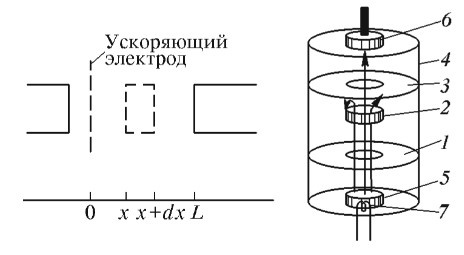
\includegraphics[scale=0.8]{../images/513-3}
\caption{Схематическое изображение тиратона (слева) и его конструкция (справа): 1, 2, 3 -- сетки; 4 -- внешний металлический цилиндр; 5 -- катод; 6 -- анод; 7 -- накаливаемая спираль}
\end{figure}

Электроны, эмитируемые катодом тиратона, ускоряются напряжением V, приложенным между катодом и ближайшей к нему сеткой. Затем электроны рассеиваются на атомах ксенона.

\section{Проведение эксперимента}

\begin{enumerate}

\item Включим блок питания в сеть и настроим установку.

\item Переключим установку в динамический режим работы. Установим напряжение накала $V_{накала}=3.383$. Оно не будет менять на протяжении всей работы.

\item Пронаблюдаем вольт-амперную характеристику тиратрона на экране электронного осциллографа.

\begin{figure}[H]
\centering
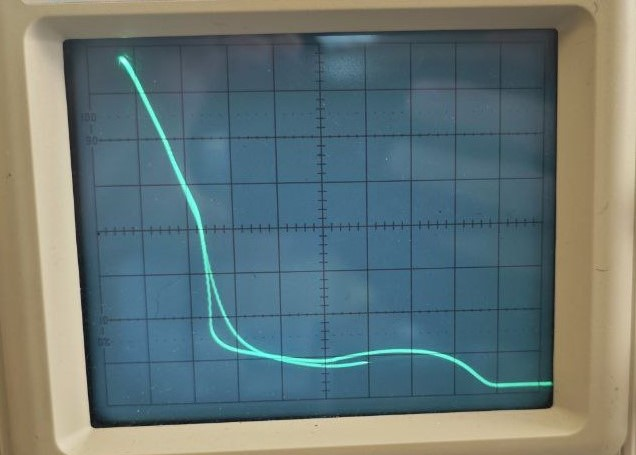
\includegraphics[scale=0.6]{../images/513-7}
\caption{Измерение ВАХ в динамическом режиме}
\end{figure}

\item Перейдем к статическому режиму измерений. Проведем подробное измерение вольт-амперной характеристики. Особенно тщательно проведем измерения в областях максимума и минимума характеристики.

\begin{figure}[H]
\centering
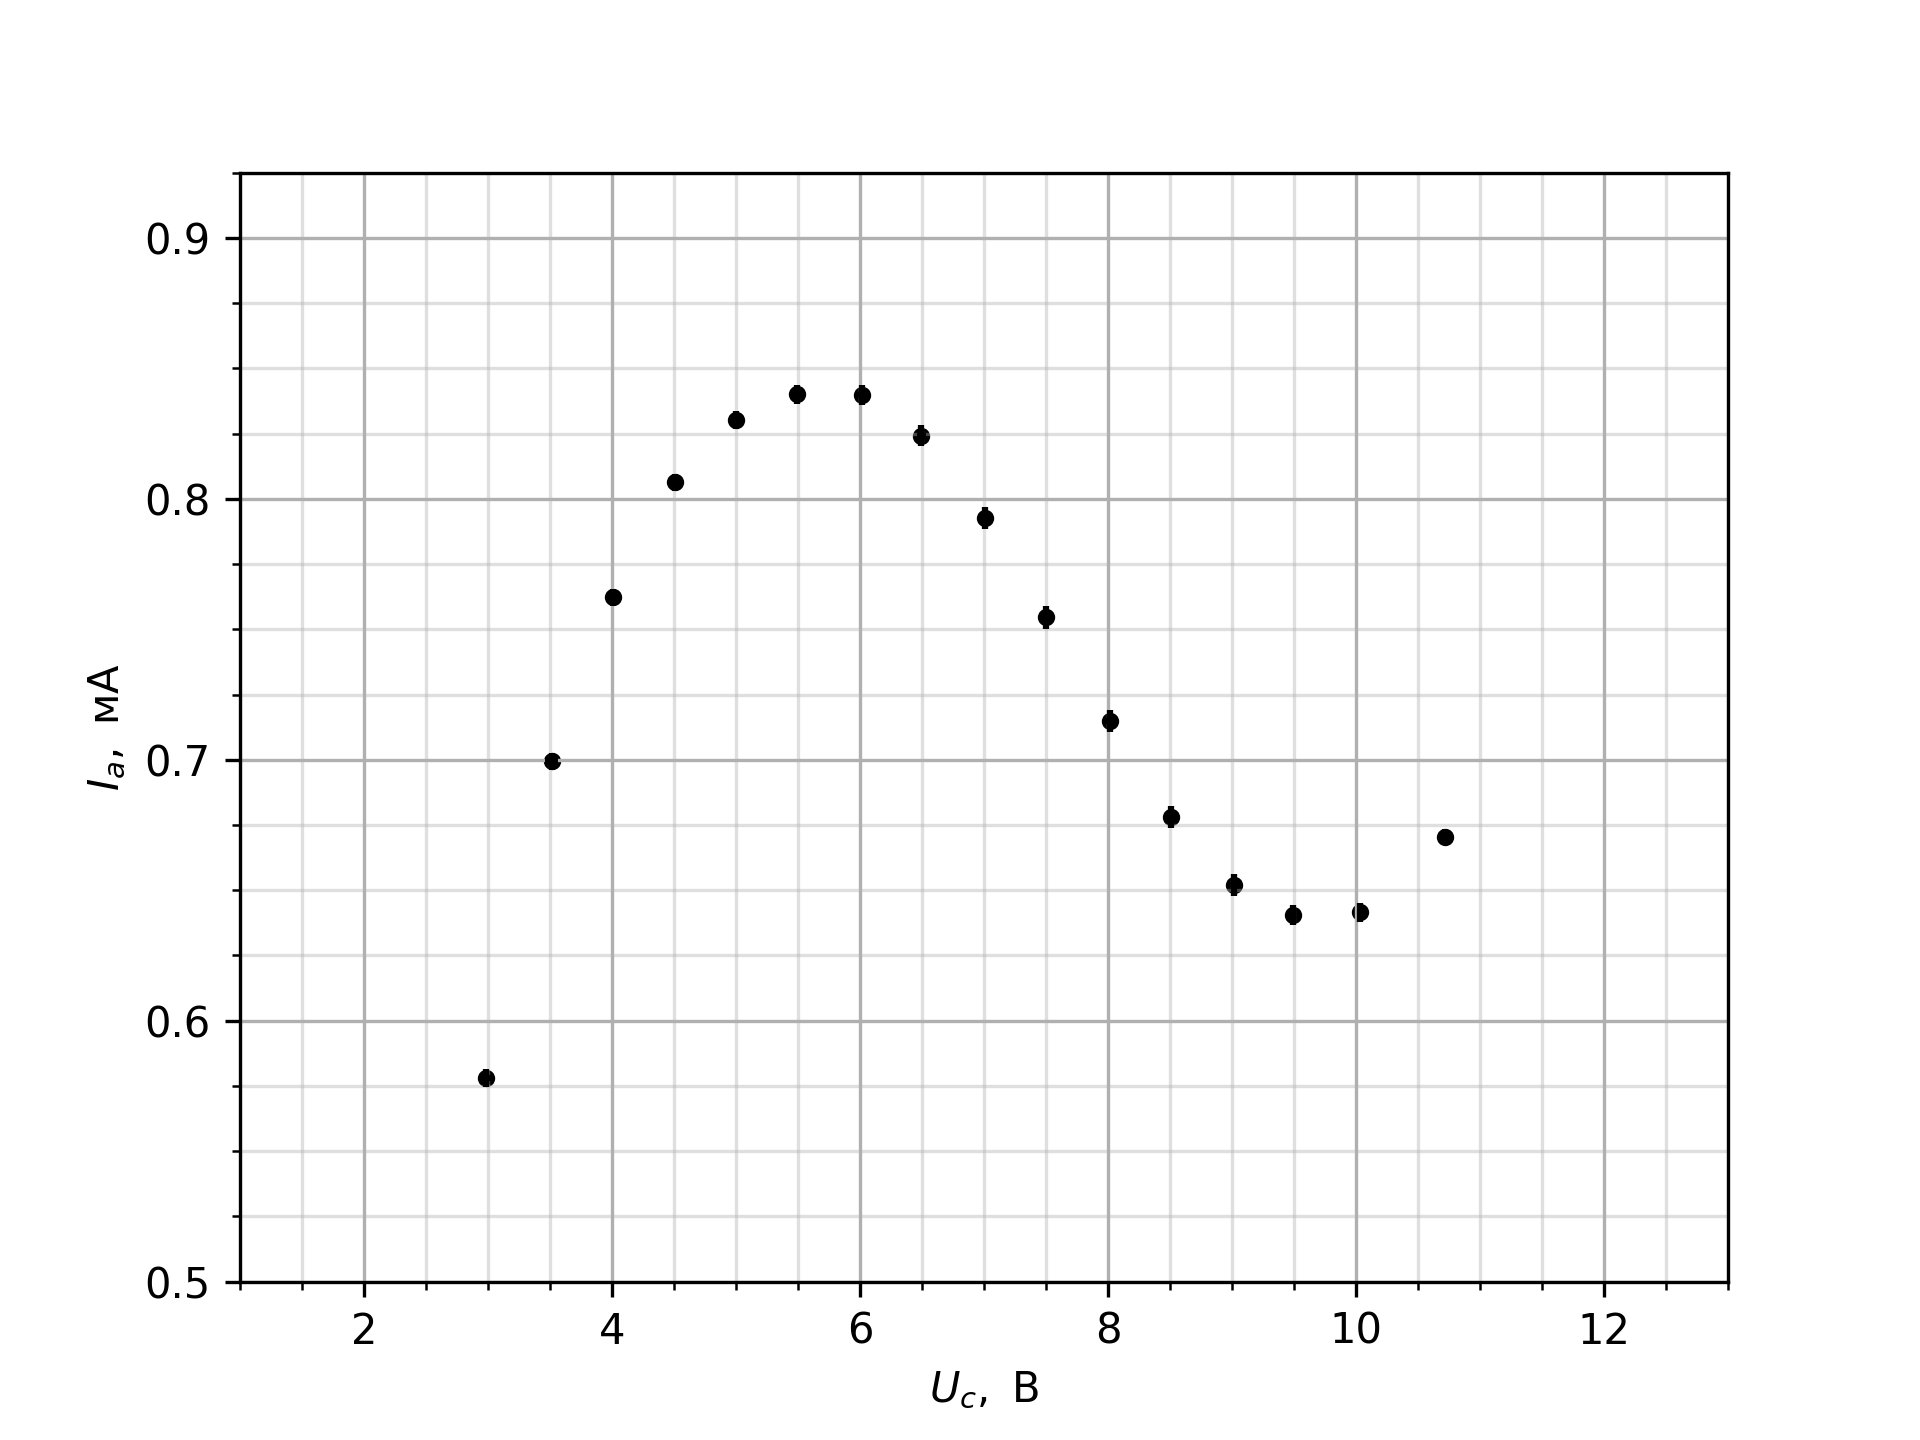
\includegraphics[scale=0.8]{../images/513-4}
\caption{Зависимость анодного тока от ускоряющего напряжения}
\end{figure}

\item Установим все ручки регуляторов в минимальное положение и отключим все приборы.

\end{enumerate}

\section{Обработка результатов}

\begin{enumerate}

\item По результатам измерений в динамическом режиме оценим размер электронной оболочки атома, приняв $U_0=2.5\ В$. Погрешность таких измерения составляет $\sigma_E\approx1\ В$.

\[E_1\approx 6\ В,\quad E_2\approx 10\ В\]

\[l_1=\frac{1}{2}\frac{h}{\sqrt{2m(E_1+U_0)}}=(2.10\pm0.12)\ \si{\angstrom}\]
\[l_2=\frac{3}{4}\frac{h}{\sqrt{2m(E_2+U_0)}}=(2.60\pm0.10)\ \si{\angstrom}\]

\[l=\frac{h\sqrt{5}}{\sqrt{32m(E_2-E_1)}}=(3.4\pm0.2)\ \si{\angstrom}\]
\[U_0=\frac{4}{5}E_2-\frac{9}{5}E_1=(-2.8\pm1)\ В\]

\item В результате измерения напряжения пробоя, получим $U_{пр}=15.5\ В$. Это примерно соответсвует потенциалу ионизации аргона, равному $U_{пр, Ar}=15.8\ В$.

\item Построим график $I_a=f(U_c)$ для статического режима. По графику определим положения экстремумов зависимости, аппроксимировав их параболами вида $I_a=k(U_c-U_в)^2+I_в$.

\begin{figure}[H]
\centering
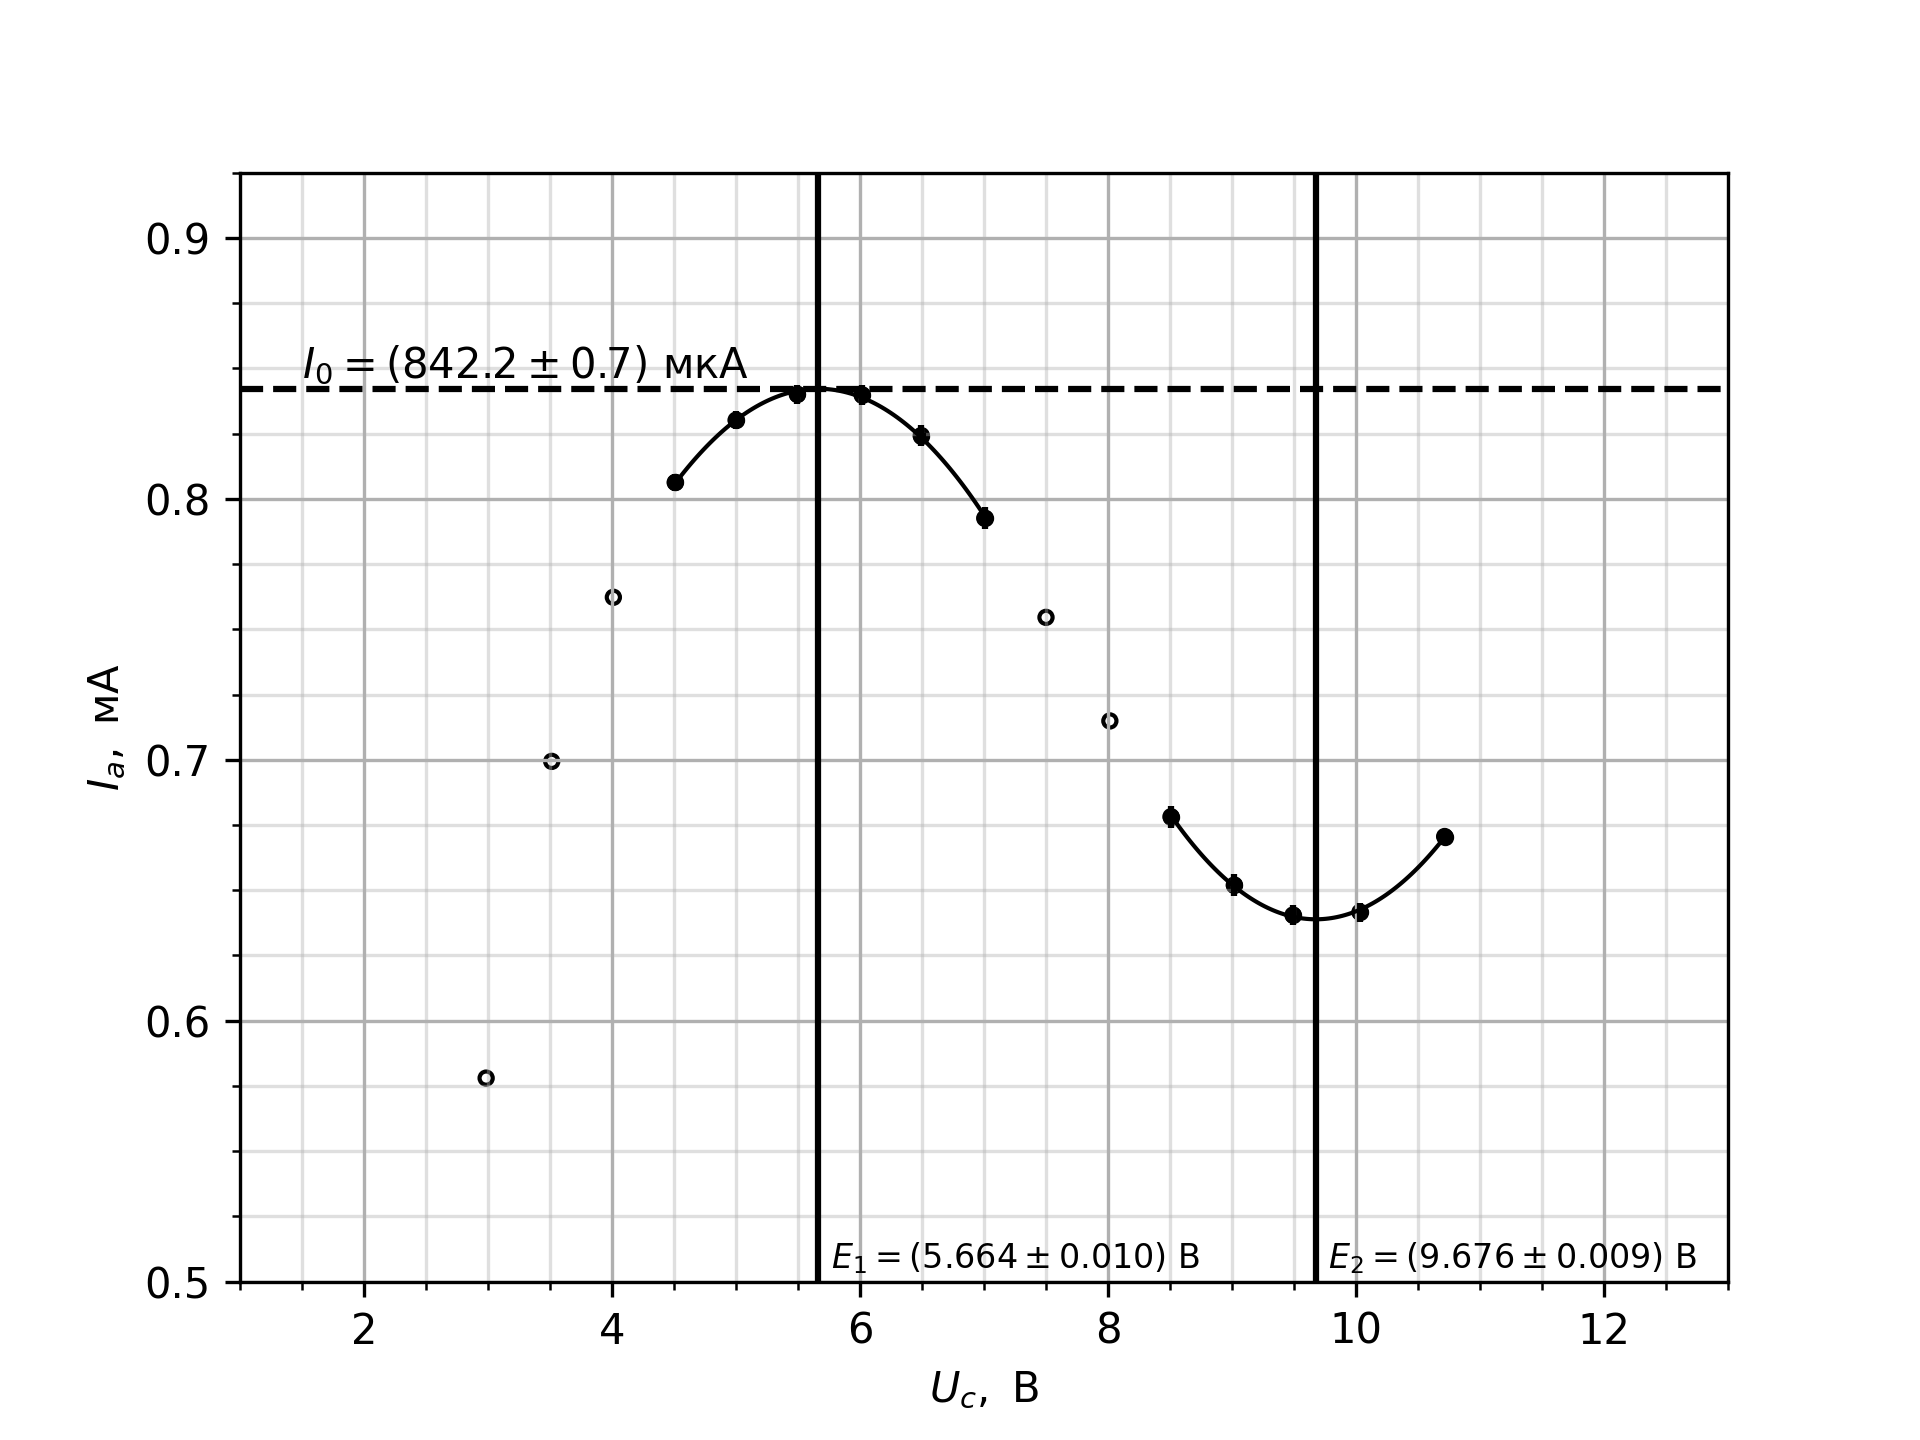
\includegraphics[scale=0.8]{../images/513-5}
\caption{Определение положения пиков ВАХ}
\end{figure}

Проведем те же расчеты, что и в динамическом режиме.
\[l_{стат}=(3.423\pm0.002)\ \si{\angstrom},\quad U_{0,\ стат}=(-2.46\pm0.04)\ В\]

Также из графика определим величину $I_0=(842\pm0.7)\ мкА$ как высоту первого экстремума.

\item Оценим при каких напряжения должны появляться максимумы в коэффициеннте прохождения электронов для $n=2,\ 3$. Для этого выразим следующую зависимость:

\[E_n=f(E_1, n)=n^2 E_1+(n^2-1) U_0\]
\[E_2=4E_1+3U_0=(15.3\pm0.2)\ В\]
\[E_3=9E_1+8U_0=(31.3\pm0.4)\ В\]

Пик анодного тока при $n=2$ на АЧХ трудно различим из-за наличия пробоя ($U_{пр}=15.5\ В$). Пик при $n=3$ в данном эксперименте пронаблюдать не удастся.

\item Найдем зависимость вероятности рассеяния электронов от энергии. Построим график зависимости

\[w(V)=-\frac{1}{C}\ln{\frac{I_a(V)}{I_0}}\text{.}\]

\begin{figure}[H]
\centering
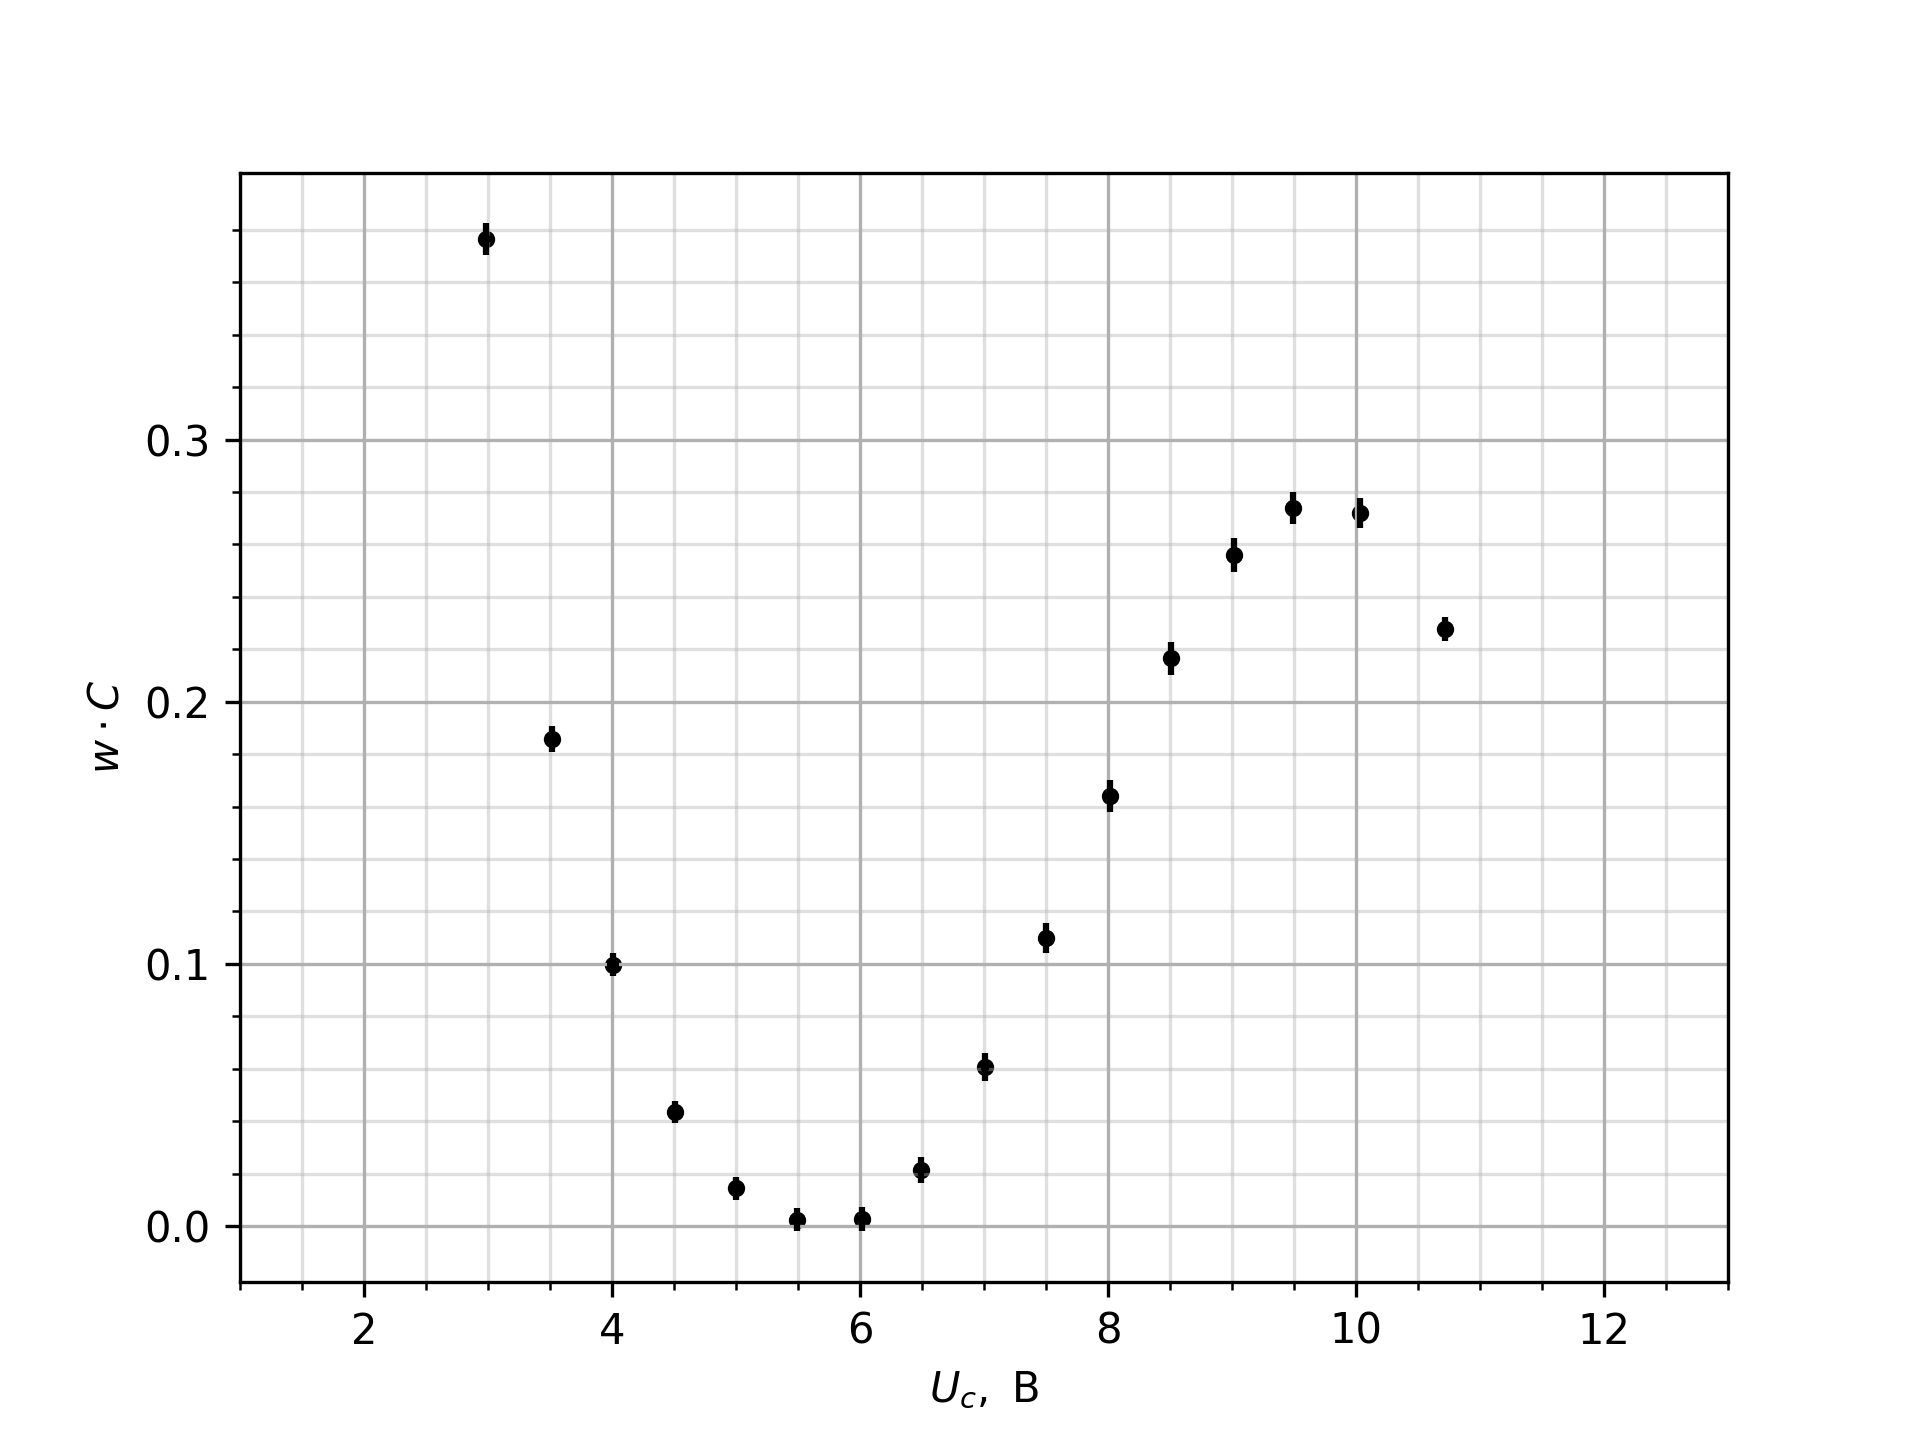
\includegraphics[scale=0.8]{../images/513-6}
\caption{График зависимсоти w(V)}
\end{figure}

\item При поднесения постоянного магнита к тиратрону изменяется его АЧХ. Пронаблюдаем изменения в динамическом режиме.

\begin{figure}[H]
\centering
\begin{subfigure}{.5\textwidth}
  \centering
  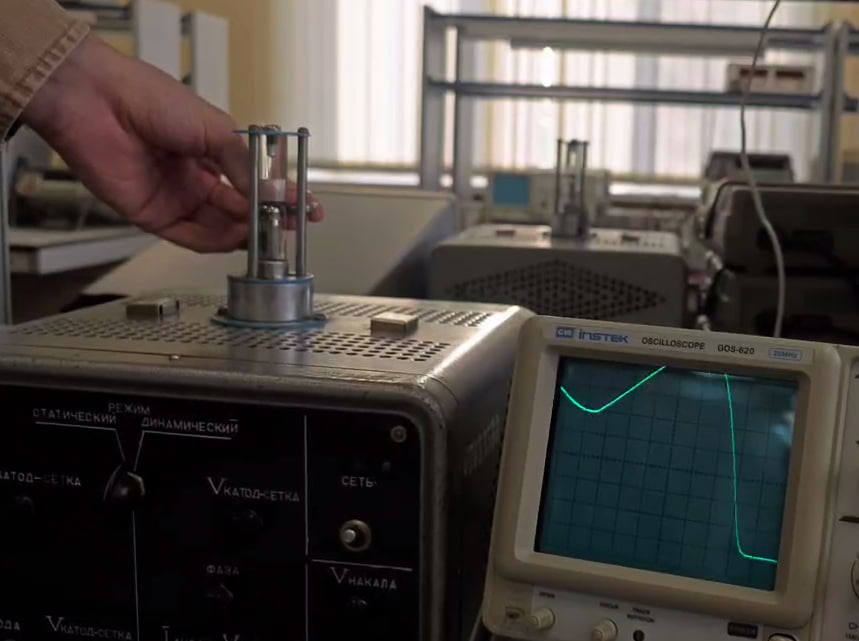
\includegraphics[width=.9\linewidth]{../images/513-8a}
\end{subfigure}%
\begin{subfigure}{.5\textwidth}
  \centering
  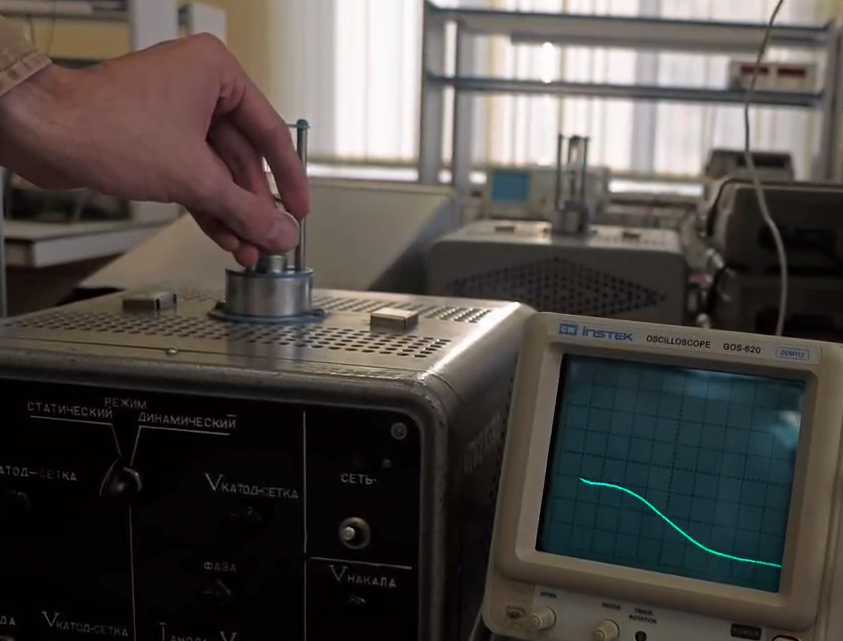
\includegraphics[width=.9\linewidth]{../images/513-8b}
\end{subfigure}
\caption{Изменения АЧХ при поднесении магнита}
\end{figure}

При соосном расположении магнита и тиратрона анодный ток заметно усиливается, а при перпендикулярной ориентации анодного тока практически нет. Данный эффект обусловлен взаимодействием движущихся электронов с магнитным полем постоянного магнита.

Определение внутреннего устроства тиратрона затруднено практическим отсутвствием документации. Единственное, что удалось найти, это данная схема. Судя по ней анод-катод тиратрона расположены перпендикулярно продольной оси устройства. 

\begin{figure}[H]
\centering
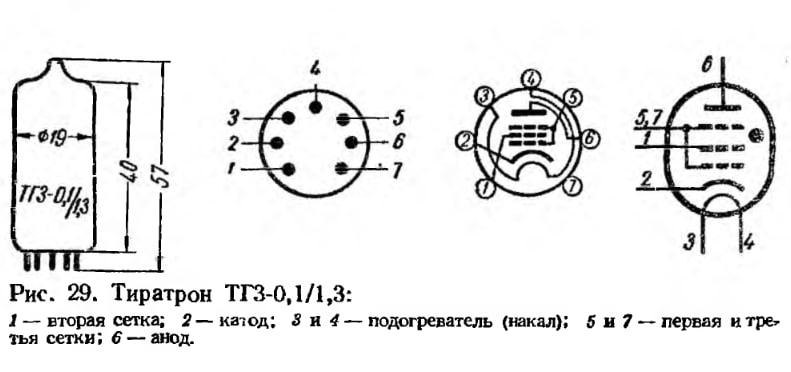
\includegraphics[scale=0.6]{../images/513-9}
\caption{Схема тиратрона ТГ3-0.1/1.3}
\end{figure}

\end{enumerate}

\section{Выводы}

В ходе работы был определен газ, наполняющий тиратрон, размер и глубину эффективной одномерной прямоугольной потенциальной ямы, соответствующей атому аргона. Обратившись к справочным данным, узнаем, что диаметр атома аргона составляет $d=3.76\si{\angstrom}$, что довольно близко к полученному размеру $l$. Крайне малые погрешности, полученные в результате выполения работы нельзя считать корректными. Неучтенные неточности модели вносят гораздо большие погрешности.

\end{document}